\section{Iterative SVM}
\begin{figure}[htbp]
\centering
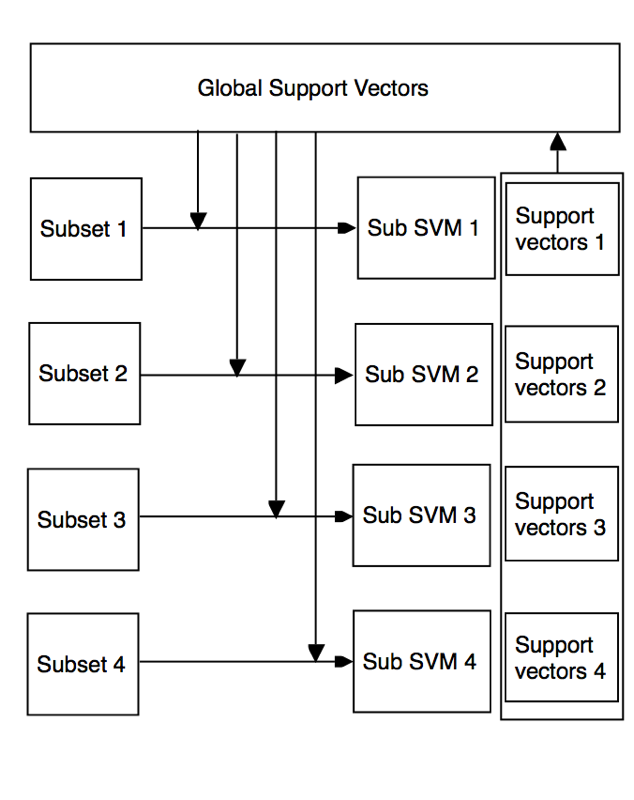
\includegraphics[width=3.0in]{image/iterativeSVM.png}
\caption{Procedure of paralleling Iterative SVM algorithm}
\label{iterativeSVM}
\end{figure}

The Iterative SVM algorithm works as Figure \ref{iterativeSVM}. The training set of the algorithm is split into subsets. Each process classifies sub dataset locally via SVM algorithm from LibSVM and gets the support vectors, and then passes the calculated support vectors to global support vectors to merge them. In Map stage of the Harp job, the subset of training set is combined with global support vectors first, and after get the new support vectors, the processes do an all-reduce to broadcast the global support vectors. And finally they can continue working on next round.

\begin{algorithm}
\caption{Iterative SVM algorithm}
\label{iterativeSVMalgorithm}
\begin{algorithmic}
\REQUIRE $dataPoints$
\ENSURE $globalSV$
\STATE split $dataPoints$ into $n$ pieces
\STATE each process gets its own piece
\STATE $globalSV=\{\}$
\FOR{$iteration=1\rightarrow n$}
\STATE combine $subDataPoints$ and $globalSV$
\STATE train data set
\STATE allreduce $SV$ to $globalSV$
\ENDFOR
\IF{Master}
\STATE output $globalSV$
\ENDIF
\end{algorithmic}  
\end{algorithm}

The pseudo code can be found in Algorithm \ref{iterativeSVMalgorithm}.